\chapter{Methodology} \label{chapter-methodology}

In this chapter we discuss the methodological approach of the thesis, as well as a number of modelling decisions. 


We are focused on the evolution of a city. In any city, numerous people and organizations in the city are making individual decisions independently, constantly adjusting in sensible ways to the changing parameters of the city they inhabit. As a result, cities evolve continuously and may never be in equilibrium.  To model this complex, dynamical, multi-agent economic system we  rely on techniques and insights from several fields and we  employ two distinct modeling approaches. We develop and explain the theoretical foundation of our work using a range of results from the economic  literature. We go on to implement the theoretical model in the agent-based modeling (ABM) framework. 
% In doing so we are attentive to the strengths and weaknesses of the approaches that we are adopting. 

\subsection{Equilibrium vs ABM modeling}

Economists rely heavily on equilibrium analysis in their study of complex systems. 
%In Economic modelling the most familiar approach is the  analysis of systems in equilibrium. 
A set of necessary conditions describing a steady state of interest are imposed and then solved to find features of the equilibrium they generate. It is a productive methodology partly because it  bypasses the complex process of adjustment, focusing on the conditions that must be true if a particular situation is to persist.

The classic example is the ubiquitous supply and demand model. Each curve represents plausible behaviours of a class of agents. A situation is unlikely to persist if either class of agents is unsatisfied with the combination of price and quantity. The model explores the combinations that satisfy the behavoural intentions of both classes i.e. are on both curves. If the two curves can be described mathematically, equilibrium prices and quantities can be derived solving the two-equation system.

The approach produces tractable models that can often be solved explicitly. To achieve tractability, it is often convenient 
to limit the number of independent decision-makers by employing a ``representative agent.'' To extend the analysis to dynamic systems, ``laws of motion'' (adjustment rules) can be added in the form of either difference or differential equations.  Models quicliy become intractable with more agents or dynamic 
processes, and economists, like other modellers, resort to simulation 
and numerical methods. 



In an \gls{ABM}, agents are defined as having adjustment rules or behaviours that respond to environmental variables.\footnote{This approach is not unfamiliar to economists - The Cournot duopoly model, for example, is analyzed using `reaction functions' which simply describe a firm's optimal response to as second firm's output choice.} 
Unlike equilibrium approaches, agent based modelling commits to using computational methods to mimic the distributed decision making of complex systems like cities. A program is written that considers each agent sequentially and updates agent and system statuses as it goes. The program is allowed to iterate, and the values of any state variables of interest are recorded at each step. The model may or may not settle into a steady state. As with other modelling approaches, ABMs can be used explore the behaviour of the system by varying individual parameters, and to explore the parameter space using Monte Carlo methods.

% In ABMs it is often makes sense to simplify models, less for computational reasons then to % The problem of model complexity remains a challenge with ABMs, however, and modellers introduce simplifying assumptions. These are not as a rule needed for the computational model but are very helpful in maintaining
% maintain a focus on the key theme  of the model.  %(ADD distinction between detailed models and detailed explicit models)

We draw heavily on existing economic analysis of cities to identify relevant behaviours and parameters. We also employ three key economic equilibrium conditions drawn from the economic literature: a locational, labour market, and a housing market equilibrium conditions
%Some adjustments are slow and some are fast. Rates of adjustment can matter. 

Because our focus is financialization in the land market, we use the equilibrium conditions for competitive labour markets to bypass the complex and partially understood wage-setting process. We assume, a core theoretical result from the theory of the firm, that workers are paid their \gls{marginal value-product}. We ground this approach in recent research that has derived and estimated an aggregate urban production function consistent with modern \gls{neoclassical growth theory}.\footnote{We are not aware of other research that has taken this step yet.} We use the result to derive an urban wage premium that drives city growth. We would argue that, since housing and labour markets can adjust more quickly than urban productivity, we can assume that they respond  continuously to the slower movement of population and productivity. % need to reference? 

A similar market-based argument allows us to assume that land rents are determined by the classic urban locational equilibrium. The theory is based on the insight that if individual utilities are higher at one location in the city, entrants or movers will choose that  location. This is an implication of consumer choice theory. In a market with any degree of churn market prices for land should converge on use values, and these will vary systematically with transportation costs. For simplicity, we present the model for the case where individuals have the same preferences, employment opportunities and transportation costs. Building on this, %In the computational model 
we can introduce site-specific and person-specific features. 

Finally, we employ \gls{equilibrium reasoning} in the housing and investment process. We assume investors behave rationally in that they estimate the potential returns on their investments and seek the highest returns they can get. They calculate an offer price in each transaction based on several factors: land rents, expected price changes, their individual price of capital and discounting rate, and the information available to them.

It is at this point we introduce an innovation to formal urban modelling. We draw on the literature for the relevant `\gls{stylized facts}' about differences in these values based on wealth and income. This opens the possibility of urban segregation and the endogenous emergence of \gls{class} distinction based on capital access, a process explored by John Roemer in his neglected General Theory of Exploitation and Class \cite{roemerGeneralTheoryExploitation1982}.  

\Gls{expectations} have to take into account some amount of current and past information. Forecasts based on recent price movements can give rise to price bubbles through either speculative or precautionary motives. Expectations anchored in \gls{perfect foresight} have different dynamics, since agents correctly forecast the path of prices. We employ backwards-looking expectation formation anchored 
%  This ANCHORING IS INTERESTING, BY THE WAY
to current rental returns, which allows agents to be misled by rapidly rising prices. We derive an investment rule of this sort in Chapter~\ref{chapter-financialization}. 

\subsubsection{Overlapping generations}
In our model individuals have a working life, then retire. If they own homes they sell and move to the countryside where housing is cheaper. They are replaced by new entrants from the countryside. New entrants may become buyers or tenants. This is a variant of the \gls{overlapping generations  model} in which savings are passed on to the next generation. In our case homes are passed on, as agents retire and move away. While the model has multiple generations, it is not a `dynastic' model in which the generations are linked by family ties and inheritance maters in individual decision-making, because the core issue in the emergence of classes is whether the city continues to provide opportunity for newcomers, and those without the benefit of generational wealth. % to share the  benefits of agglomeration effects. % to share in the . %We suspect that introducing families would complicate the model but add little to understanding  our  main  issue. 

\subsubsection{Urban and rural wages}
A modelling device that plays a major role is our use of the \gls{urban wage premium}, the difference between a rural and an urban wage driven by positive agglomeration effects on productivity in the city. It cannot be competed away because transportation costs limit access to the productive centre. The wage premium is a partial measure of the agglomeration effect. It generates the \gls{rent premium} on urban land. We want to call attention to the distribution of that rent premium.

To simplify the analysis, we assume that we can partition actual wages between the wage premium, which is available for accumulation or spent on transportation, and all other expenses. We assume urban and non-urban populations all receive a \gls{subsistence wage} which covers  the cost of buildings, food and other living costs and a base cost of land.\footnote{This base cost appears in other models as the cost of agricultural land. It is more precisely described as the opportunity cost of rural land. We simply extended the technique to include the opportunity cost of urban labour, allowing us to focus on the rents themselves.} 

There are advantages and disadvantages to this technique. The motivating advantage is that it lets us isolate the social surplus generate by agglomeration. One disadvantage is that it suppresses many issues that are of interest in other contexts - such as choice of home size and quality. In the computational model it is easy to allow for different building types and more complex housing choice, but in this section we simply  want to make the logic of our model as clear as possible. We foresee adding layers to the computation model that incorporate redevelopment and construction and allow for decisions about scale, type and location. 

Another disadvantage of technique in the analytical version is that it does not allow us to make speculation on  the value of  buildings part of our market process. It is a problem that can be dealt with in the computation model, but we believe the added complexity will not add to our central argument. Research (see \cite{mcdonaldWilliamAlonsoRichard2007}) has shown  that the core model is robust to many extension of this sort. 

\subsubsection{Examples of  \gls{equilibrium} reasoning in our analysis}
As an example of \gls{equilibrium reasoning},  we implicitly impose the locational equilibrium condition,
\[U_i(d,\dots)=U_j(d, \dots)\]
This says that identical individuals must get the same utility living at at whatever distance from the city centre. If that were not the case, individuals would move to a location where they get higher utility. For utility to remain constant as $d$, and therefore transportation costs  rise, some other variable must compensate. In this class of models, rent charged for the use of land must fall as distance increases. Equilibrium locational choice by commuters therefore determines the extent and even population of the city.\footnote{More complex models allow home sizes and lot sizes in the suburbs to increase as well.} Since land value  is capitalized rent, land values also decline toward the edge of the city until they are equal to the rural value of land, 
% different location would take a long time to work through the system. Prices, however, can adjust much more quickly. 

An adjustment process that requires people to move to a different location would take a long time to work through the system. Prices, however, can adjust much more quickly.



%  It follows that 
% \[\frac{\partial U_i(d, d(dots)}{\partial t}=\frac{\partial U_j(d, /dots)}{\partial t}\]
% With identical transportation cost, 
% land rents are determined by transportation costs  

We also rely on equilibrium arguments in our model to ``black box'' the productions sector and most of  the labour market, including most decisions by producers and wage demands by workers. 

% More recent work has looked at agent-based modeling, looking at the dynamics, space and individual work. 


\subsubsection{\Gls{marginal} vs \gls{inframarginal} quantities}

In relying on these equilibrium conditions, we are implicitly applying standard neoclassical economic methods despite the fact that our focus is not on the \gls{marginal} conditions that determine prices, but on the \gls{inframarginal} quantities that make up rents. We can illustrate with a diagram that is more fully explained in Chapters~\ref{chapter-rent} and \ref{chapter-space}. 

\begin{figure}[hb]
    \centering
  
 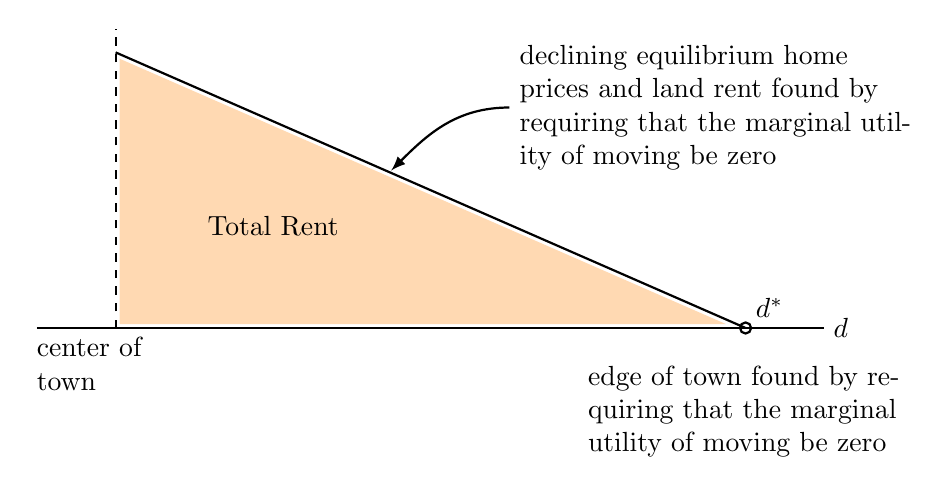
\begin{tikzpicture}[domain=0:2]
%\draw[thick,color=gray,step=.5cm, dashed] (-0.5,-.5) grid (3,3);
\draw[line width=.01] (0,0) -- (10,0) node[right] {$d$};
\node at (1,0) [below,text width=2cm] {center of town};
%\draw[thick ] (0,3)node[above right] {merchant's price in town} -- (10,3) ;
\draw[thick ] (0,0)  -- (10,0); 

\draw[thick, -latex] (6,2.8)
node[right, text width=5cm]{declining equilibrium  home prices and land rent found by requiring that the marginal utility of moving be zero} 
to [out=180, in=45](4.5,2); 

\fill[orange!30] (1.05,0.05)--(8.75,0.05)--(1.05,3.42)--cycle;

\draw[thick, dashed ] (1,0) -- (1,3.8);
\draw[thick ] (9,0)node [above right]{$d^*$}circle[radius=2pt] node[below=.35cm,text width=4cm] {edge of town found by requiring that the marginal utility of moving be zero} -- (1,3.5) ;

\node at (3,1.3){Total Rent};
\end{tikzpicture} 
   \caption{Marginal and infra-marginal quantities}
    \label{fig:landrentasinframarginal}
\end{figure}
In Figure \ref{fig:landrentasinframarginal}, The level of rent is determined at any distance by individuals making comparison very locally. At point $d^*$ the person at the edge of the city decides whether to work in the centre or in the non-urban space. These are \gls{marginal} decisions. The orange area represents  the total rents generated between $d=0$ and $d=d^*$. It is a summation of \textbf{\gls{inframarginal}} rents. Like Ricardo in his classic study \cite{ricardoEssayInfluenceLow1815}, we are concerned with the distribution of rents, which are an  inframaginal quantity.


providing tractable models.  equilibrium analysis of marginal effects, and representative agents which hid distributional effects, as well as spaceless economic models of markets made it difficult to capture the richer spacial dynamics of urban rents, and the details of the ways economic forces play out for individual actors.

First they've not tended to build in, in a sophisticated way classical economic theory,
In general, classical economic theory has not been developed in agent based modeling work
Agent based models have begun with simple models, using and relaxing neoclassical assumptions, and building from first principles. This is absolutely the place to start. As the field matures, it makes sense to introduce theory in a more nuanced way, that connects with classical theory/the history of thought, etc

Second, relatively little agent based modelling work integrates with the neoclassical economic work in a way that makes the relation clear/holds the advantages. ABM work tends to both reject neoclassical approaches and rely on neoclassical assumptions.
More generally only a few agent models (e.g. spruce budworm) connect the analytic and agent models in a clear rigorous way. We focus on holding in addition to the relation with classical theory, a close connection with the many advances made withing neoclassical modelling

- this connection will make it easier to incorporate in teaching and for mainstream economists to engage on and build with.

This work builds, first, a simple conceptually clear model tightly integrated with the core economic modelling traditions, that builds on the theory of rent.

% ALSO (Agent modelling also tents to model individuals- we also take some steps to agent based modelling beyond the individual, and to the work developing model in a mode ideas)

Third, econ lacks resilience analysis and models, yet hysteresis clearly present in the relation between the built environment and econ activity. Although there's been work on dynamics and individual effects, there has been little work looking at the resilience dynamics in economic models, we take that approach looking at the resilience of community and individual wealth, and the relationship between that wealth and productivity. 

- This puts resilience dynamics at the center of economic analysis.

The resilience analysis looks at the dynamics of rent in economic boom and bust cycles.
There is a ratchet effect, achieved through hysteresis in the system, in which sucks wealth out of communities on the way up and on the way down. % DETAIL ONCE DRAFTED.


\section{Other notes - to sort}

% TEMP - here are some other notes we may want to reference or bring in. [[non individualistic modeling of agents]] [[generalizability in agent vs classical econ models]]

The emphasis is on clarity and connecting with the equilibrium in economics, and systematically relaxing each, to connect with the analytic tradition of economic modelling
The clarity of intuition of the neoclassical tradition with the deeper root of distribution theory rooted in classical economics and the breath and rigor possible with new tools from the study of complexity and statistical physics.

Methodological questions: 

    - agent models (integrating theory more completely into agent models)
    
    - rent theory

Core model

    - static version
    
    - dynamic version

Simulations
Result - hysteresis,
Policy
